
% Setup
    \documentclass[a4paper, 10pt, conference]{ieeeconf}
    \IEEEoverridecommandlockouts                              % This command is only
                                                              % needed if you want to
                                                              % use the \thanks command
    \overrideIEEEmargins
    % See the \addtolength command later in the file to balance the column lengths
    % on the last page of the document

    \usepackage[utf8]{inputenc}
    \usepackage[T1]{fontenc}
    \usepackage{xcolor}
    \usepackage[
bibstyle=ieee,
isbn = false,
doi = false,
url = false,
eprint=false]{biblatex}


\AtEveryBibitem{\clearfield{address}}
\AtEveryBibitem{\clearlist{language}}

\addbibresource{refs.bib}

\DefineBibliographyStrings{english}{
  phdthesis   = Ph\adddot D\adddot\addspace thesis,
  mathesis    = Master's thesis,
}

% https://ftp.snt.utwente.nl/pub/software/tex/macros/latex/contrib/biblatex-contrib/biblatex-ieee/ieee.bbx

%swapped chapter+pages with published+location date:

\DeclareBibliographyDriver{inproceedings}{%
  \usebibmacro{bibindex}%
  \usebibmacro{begentry}%
  \usebibmacro{author/translator+others}%
  \setunit{\labelnamepunct}\newblock
  \usebibmacro{title}%
  \newunit
  \printlist{language}%
  \newunit\newblock
  \usebibmacro{byauthor}%
  \newunit\newblock
  \usebibmacro{maintitle+booktitle(inproceedings)}%
  \midsentence
  \newunit\newblock
  \usebibmacro{event+venue+date}%
  \newunit\newblock
  \usebibmacro{byeditor+others}%
  \newunit\newblock
  \printfield{volumes}%
  \newunit\newblock
  \usebibmacro{series+number}%
  \newunit\newblock
  \printfield{note}%
  \newunit\newblock
  \printlist{organization}%
  \newunit\newblock
  \usebibmacro{volume+part}%
  \newunit\newblock
  \usebibmacro{chapter+pages}% %swapped chapter+pages with published+location date
  \newunit
  \usebibmacro{publisher+location+date}%
  \newunit\newblock
  \iftoggle{bbx:isbn}
    {\printfield{isbn}}
    {}%
  \newunit\newblock
  \usebibmacro{doi+eprint+url}%
  \newunit\newblock
  \usebibmacro{addendum+pubstate}%
  \setunit{\bibpagerefpunct}\newblock
  \usebibmacro{pageref}%
  \newunit\newblock
  \iftoggle{bbx:related}
    {\usebibmacro{related:init}%
     \usebibmacro{related}}
    {}%
  \usebibmacro{finentry}}
  
  
  %swapped chapter+pages with published+location date:
  
  \DeclareBibliographyDriver{incollection}{%
  \usebibmacro{bibindex}%
  \usebibmacro{begentry}%
  \usebibmacro{author/translator+others}%
  \setunit{\labelnamepunct}\newblock
  \usebibmacro{title}%
  \newunit
  \printlist{language}%
  \newunit\newblock
  \usebibmacro{byauthor}%
  \newunit\newblock
  \usebibmacro{in:}%
  \usebibmacro{maintitle+booktitle}%
  \newunit\newblock
  \usebibmacro{series+number}%
  \newunit\newblock
  \usebibmacro{byeditor+others}%
  \newunit\newblock
  \printfield{edition}%
  \newunit
  \iffieldundef{maintitle}
    {\printfield{volume}%
     \printfield{part}}
    {}%
  \newunit
  \printfield{volumes}%
  \newunit\newblock
  \printfield{note}%
  \newunit\newblock
  \usebibmacro{chapter+pages}%
  \newunit\newblock
  \usebibmacro{publisher+location+date}%
  \newunit\newblock
  \iftoggle{bbx:isbn}
    {\printfield{isbn}}
    {}%
  \newunit\newblock
  \usebibmacro{doi+eprint+url}%
  \newunit\newblock
  \usebibmacro{addendum+pubstate}%
  \setunit{\bibpagerefpunct}\newblock
  \usebibmacro{pageref}%
  \newunit\newblock
  \iftoggle{bbx:related}
    {\usebibmacro{related:init}%
     \usebibmacro{related}}
    {}%
  \usebibmacro{finentry}}


    % The following packages can be found on http:\\www.ctan.org
    \usepackage{graphics} % for pdf, bitmapped graphics files
    \usepackage{epsfig} % for postscript graphics files
    \usepackage{mathptmx} % assumes new font selection scheme installed
    \usepackage{mathptmx} % assumes new font selection scheme installed
    \usepackage{amsmath} % assumes amsmath package installed
    \usepackage{amssymb}  % assumes amsmath package installed

    \title{\LARGE \bf
    Experimental Validation of Reference Spreading by Robotic Manipulation of Unmodeled Objects
    }

    %\author{ \parbox{3 in}{\centering Huibert Kwakernaak*
    %         \thanks{*Use the $\backslash$thanks command to put information here}\\
    %         Faculty of Electrical Engineering, Mathematics and Computer Science\\
    %         University of Twente\\
    %         7500 AE Enschede, The Netherlands\\
    %         {\tt\small h.kwakernaak@autsubmit.com}}
    %         \hspace*{ 0.5 in}
    %         \parbox{3 in}{ \centering Pradeep Misra**
    %         \thanks{**The footnote marks may be inserted manually}\\
    %        Department of Electrical Engineering \\
    %         Wright State University\\
    %         Dayton, OH 45435, USA\\
    %         {\tt\small pmisra@cs.wright.edu}}
    %}

    \author{Gijs van den Brandt% <-this % stops a space
    % \thanks{*This work was made in accordance with the TU/e Code of Scientific Conduct for the Master thesis}% <-this % stops a space
    % \thanks{$^{1}$H. Kwakernaak is with Faculty of Electrical Engineering, Mathematics and Computer Science,
    %         University of Twente, 7500 AE Enschede, The Netherlands
    %         {\tt\small h.kwakernaak at papercept.net}}%
    % \thanks{$^{2}$P. Misra is with the Department of Electrical Engineering, Wright State University,
    %         Dayton, OH 45435, USA
    %         {\tt\small p.misra at ieee.org}}%
    }

  \usepackage{pdfpages}

    \begin{document}


  % 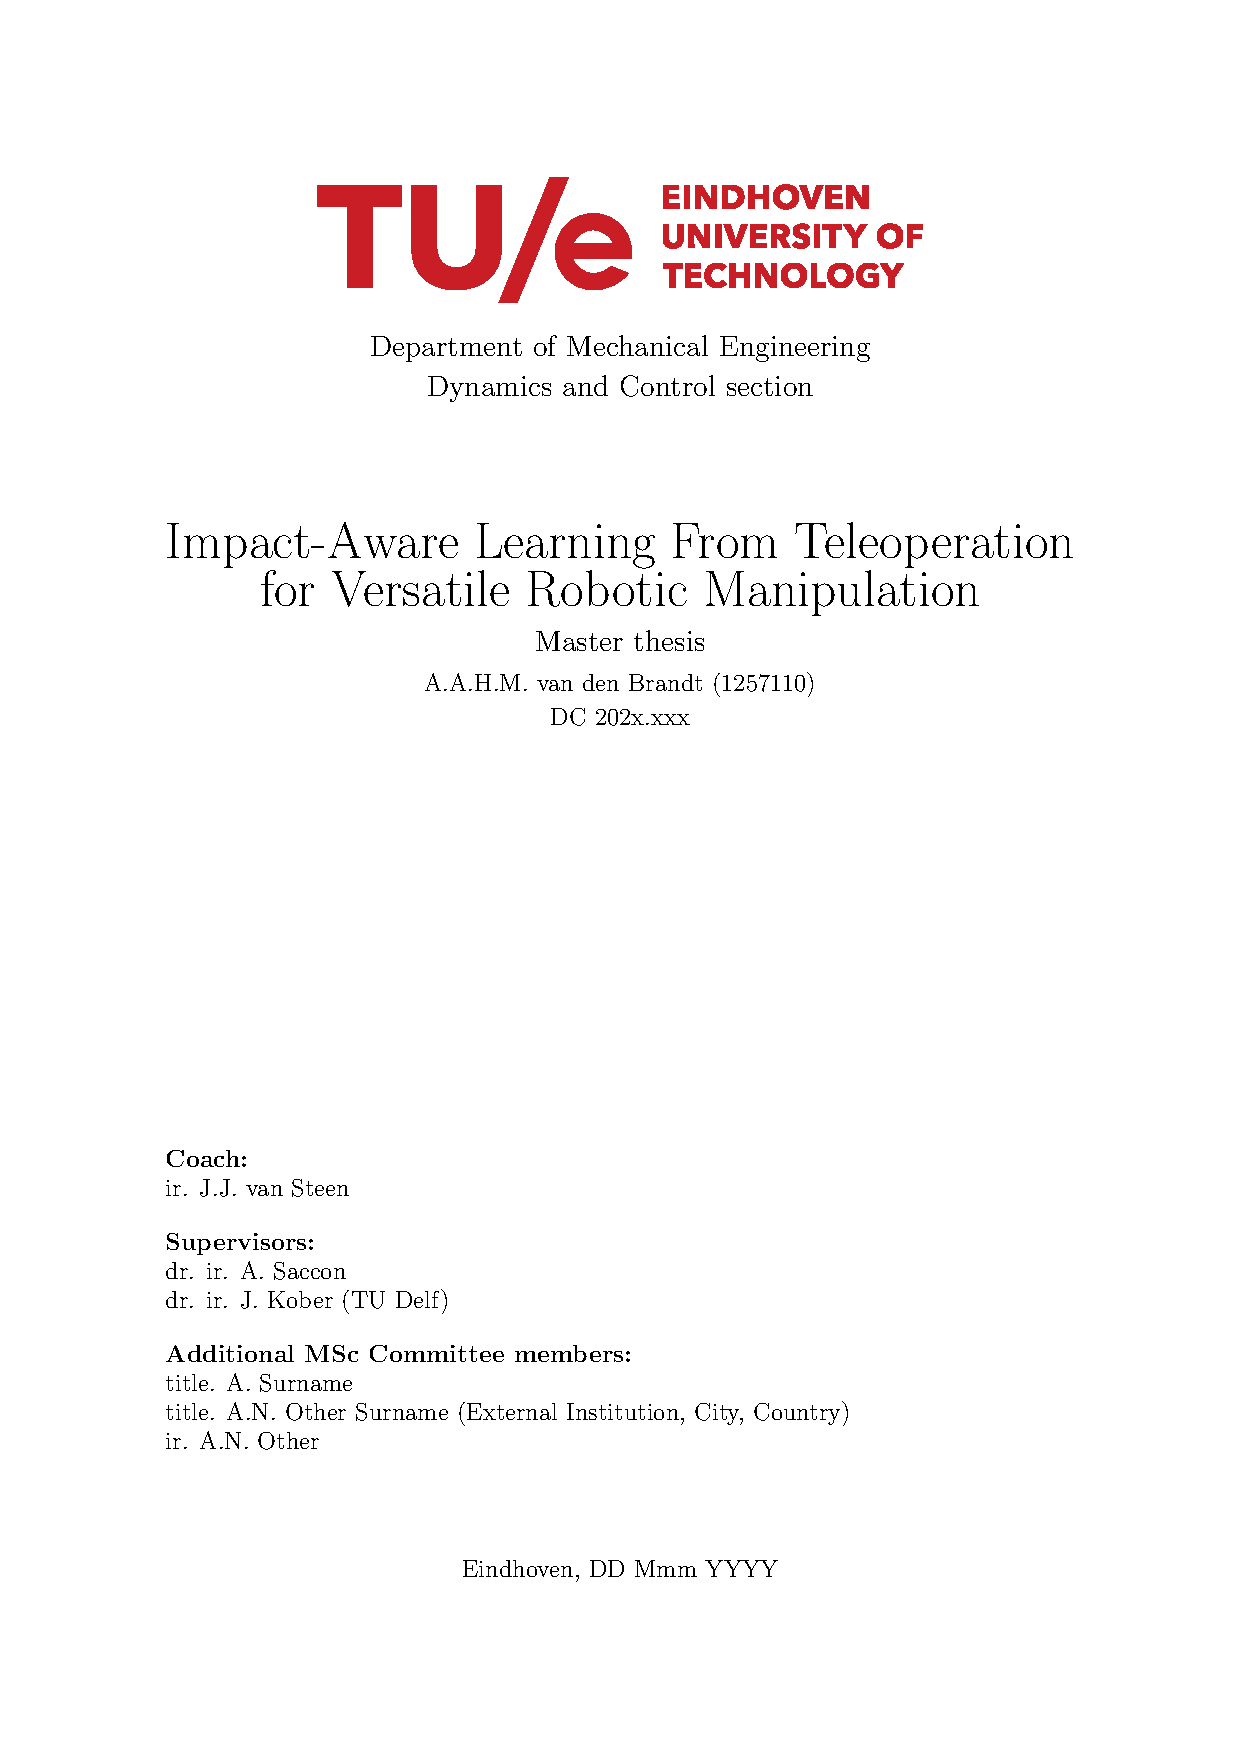
\includepdf{Thesis.pdf}
    \maketitle
    \thispagestyle{empty}
    \pagestyle{empty}

% Abstract
    \begin{abstract}

    Exploiting impacts can speed up robotic object manipulation.  However,  when using traditional control approaches, impacts are paired with peaks in joint torques and contact forces that may damage the robot or its environment. Reference spreading (RS) is an impact-aware control approach that addresses these peaks without significantly compromising on tracking performance. Numerical studies have validated the benefits of RS controllers for object manipulation tasks, but these controllers rely on knowledge regarding the robot's contact state and accurate object models --  information that is not easily available in a real-life setup. 

    To facilitate experimental validation of RS for object manipulation, this work describes an impact detection algorithm and a model-free trajectory planner using teleoperation. Furthermore, a soft end effector is designed. These components are implemented on a dual-arm robotic setup to evaluate RS in a usecase that is relevant to industry, namely grabbing a box. Experiments show that RS reduces control effort -- and therefore joint torques and contact forces -- without inhibiting tracking performance. Consequently, impacts at higher velocities become feasible, meaning that RS can contribute to faster object manipulation.

    \end{abstract}

% Introduction
    \section{INTRODUCTION}

    Automation has historically played a crucial role in the logistics industry. Our current way of living depends on autonomous systems for global transportation and warehousing. The growing labor shortage and increasing demand for online retail motivate further developments in the logistics sector~\cite{dekhneAutomationLogisticsBig2019}.

    % An example of automation in logistics can be found in depalletizing, where object are removed from a pallet. Three different depalletizing approaches can be found in industry. 

    A logistical aspect where machines struggle to fully compete with humans is object manipulation. A practical examples of this is depalletizing. While robots are strong and consistent when manipulating objects, humans are versatile and swift. Robots are held back from faster performance because they must often slow down prior to making contact; establishing contact at a high velocity -- an event referred to as an impact -- could cause damage to the robot or its environment. On the contrary, humans intrinsically exploit impacts in the form of grabbing, bouncing and hitting. % \textcolor{red}{(give better explanation of depalletizing: manual and automatic approach)}

    The field of impact-aware control aims to better equip robots for making contact at high velocities. These impacts are paired with large contact forces that could damage the system. Previous work describes control using the maximum allowable impact velocity that complies with safety constraints such as limits for the contact force~\cite{dehioRobotSafeImpactsSoft2021, dehioDualArmBoxGrabbing2022}. This was combined with a compliant cover for the robot that reduces contact forces at impact, facilitating higher feasible impact velocities. Rather than using a soft cover, low impact forces may also be achieved by designing a robot with low inertia and high backdrivability as was done in \cite{songDevelopmentLowInertiaHighStiffness2018}.

    In addition to the large contact forces, a subject of interest is the velocity jump at the time of impact. Time misalignments between velocity jumps in the reference and in the actual system cause the velocity tracking error to peak\cite{biemondTrackingControlMechanical2012}. This error peak results in undesired control effort and consequently increased joint torques and contact forces, which may damage the robot or its environment. Increased control effort due to error peaking should thus be avoided.

     In \cite{yangImpactInvariantControl2021}, the robot's velocities are projected into an impact-invariant subspace based on the expected point of impact. As a result, impact-driven peaks in the velocity tracking error are reduced significantly. It is not always possible to describe a point of impact, however. Often times, impacts occur between surfaces rather than just points. Furthermore, corners of the surface may impact at diverging intervals in uncertain order during what is called near-simultaneous impacts.

    The impact-aware control scheme called Reference Spreading \cite{sacconSensitivityAnalysisHybrid2014} also adresses error peaking caused by misaligned impacts. It operates on the basis of a tracking error that switches from an ante- to a post impact reference once an impact is detected. Near-simultaneous impacts can be accounted for by an intermediate impact mode as was done in \cite{vansteenRobotControlSimultaneous2021}. By addressing the peaking error, reference spreading facilitates faster object manipulation, making it interesting to industry if its effectivity can be proven in practice. 

    Experimental validations of reference spreading have been limited to interaction with a fixed environment \cite{rijnenReferenceSpreadingTracking2020,uitendaalTeachingRobotsInteraction2022}. In numerical studies, it has already been shown that reference spreading can also benefit object manipulation \cite{vansteenRobotControlSimultaneous2021,zwartImpactAwareLearningDemonstration2019}. These works use models of the environment to formulate a trajectory with impact-driven velocity jumps that are coherent with the system's dynamics. A lack of sufficiently accurate object models in the real world means that a different approach to trajectory formulation is required. Furthermore, the controllers used in simulation rely on information, such as contact state or object location, that often is not available on an experimental setup.

    The goal of this work is to \textbf{evaluate reference spreading for practical object maniulation tasks on an experimental setup.} To this end, a soft end effector is designed to increase friction during object manipulation. This end effector also reduces peaks in contact forces upon impact. Furthermore, since the lack of acurate environment models does not allow for model-based trajectory planning, a motion planner that utilizes teleoperation is formulated. To monitor the contact state using sensor data, a novel impact detector is described and compared to impact detectors from literature that are prone to false-positives. Finally, these components are implemend with a reference spreading controller on a dual-arm setup. A box-grabbing experiment is then conducted to compare control approaches with and without reference spreading.

        % \textbf{1. Motion planning for impacts without object models}: Generating a reference with velocity jumps that is coherent with the system's dynamics is challenging. 
        % One approach maps the ante-impact velocity to the post-impact velocity based on conservation of momentum [ref for impact map]. This requires a model of the environment, which is feasible in simulations with simplified dynamics, but challenging in reality.
        % Impact-driven velocity jumps could instead be inferred experimentally. In previous studies \cite{aouajPredictingPostImpactVelocity2021}, the control gains are reduced to zero upon detection of the impact while inferring an impact map, so that the velocity jump would not result in excessive motor torques.
        % A different model-free motion planning strategy is proposed, which not only produces velocity-reference jumps that are coherent with the system dynamics, but also leverages human intuition to generate fluid motions before and after the impact. This is achieved by introducing a human in the loop by means of teleoperation. %(This strategy introduces a human in the loop by means of teleoperation; the operator performs a demonstration, after which a reference can be extracted. During the demonstration, the control gains are relatively low. This mitigates the torque jumps at the time of impact, meaning that the controller does not need to be turned off. The teleoperator instinctively accounts for the low control gains and can perform precise motion tasks despite poor tracking of the controller.)

        % \textbf{2. Impact detection}: The reference spreading scheme should switch between ante-, intermediate-, and post-impact references at the appropriate time. This requires an impact detection algorithm. Approaches in literature look either at position data \cite{rijnenMotionSignalsVelocity2018} or external force estimations \cite{uitendaalTeachingRobotsInteraction2022,properAimAwareCollisionMonitoring2021,properValidationNumericalSimultaneous2022} for signs that could be caused by impacts. We show that these signs are necessary, but not sufficient conditions for an impact -- only looking at position or contact force can result in false positives. To limit false detection of impacts, a novel impact detector that looks at both force and position data is proposed and evaluated.

        % \textbf{3. Custom end effector:}

        % \textbf{\textcolor{red}{(4. Intermediate impact phase controller:)}}

% Background
    \section{Background}
    \subsection{Robots suitable for impacts}
    \textcolor{red}{goal: Explain why franka emika robot is suitable for impacts, explain torque control, show custom end effectors from literature, motivate design of a new end effector}\\
    Traditionally, robots employ low-level controllers which govern a motor torque based on a joint position or velocity reference, encoder measurements, and gain parameters. 
    % Impedance describes the relation between a motion enforced on a body and the resulting force. An example of a motion being enforced is a collision; two bodies cannot pass through each other, and this is governed by a contact force whose magnitude depends on the impedance of the bodies. To prevent high contact forces that might lead to damage during impacts, robots should have a low impedance, i.e., they should be compliant, have little internal friction, and have a low inertia.

    % The research robot LIMS2 meets the requirements for a low-impedance robot. Rather than using gearboxes, it uses a pulley system. Eliminating gearboxes reduces the main source of internal friction for traditional robots. Furthermore, the pulley system allows for the bulk off the mass -- namely the motors -- to be moved closer to the robot base, reducing the inertia. The absence of friction makes the robot backdrivable, meaning that the compliance can be controlled by the motors.





    
    \subsection{Quadratic programing control}
     \textcolor{red}{goal: motivate QP control, formulate carthesian impedance task, posture task, and list dynamics of motion and safety constraints }\\
     Controlling a robot for object manipulation involves, e.g., adressing redundancy and acounting for limits of the robot, while simultaneously applying a contact force and moving to a position. These objectives often clash with each other, meaning that they cannot always be perfectly satisfied. It is possible to distinguish between constraints -- control objectives that must always be satisfied -- and tasks -- objectives that should be performed as good as possible but not necesarily perfectly.

     Quadratic Programming (QP) relies on this philosophy. In a QP scheme, constraints and task errors are defined as a linear function of optimization parameters. Then it becomes possible to efficiently find the parameters that minmize the task errors while adhering to the constraints. Furthermore, priority between the tasks can be achieved by assigning weights. 
     In the context of a robot where the optimization parameters are, for example, joint accelerations $\ddot{q}$, the optimization problem can be formulated as

     \begin{equation}
     \min_{\ddot{q}\in\chi}\sum_i w_i \left \| e_i(\ddot{q}) \right \|^2
     \end{equation}
     where $w_i$ and $e_i$ are the respective weight and error of the task with index $i$, and $\chi$ is the feasible space where all constraints are met. The remainder of this section describes constraints and tasks that are relevant for object manipulation.

     \textbf{Torque constraint:} To protect the robot, we can define a constraint that limits the control torque $\tau$ within a safe range, i.e.,
     \begin{equation}
       \tau_{min} \leq\tau \leq  \tau_{max} 
     \end{equation}
     This constraint must be formulated as a function of optimization parameter $\ddot q$ to be compatible with the QP scheme. The relation between $\ddot{q}$ and $\tau$ is given by the equations of motion
     \begin{equation}
        M\ddot{q}+h=\tau
     \end{equation}    
     with inertia matrix $M$ and vector of gravity, centrifugal, and Coriolis terms $h$. Subsequently, the torque constraint formulated as linear function of the optimization parameter becomes
    \begin{equation}
     \tau_{min} \leq M\ddot{q}+h \leq  \tau_{max}.       
     \end{equation} 

     \textbf{Impedance task:} When manipulating objects, both the position and the contact force of the robot should be controlled. Impedance relates displacement to force, meaning that enforcing a desired impedance is a suitable control approach for object manipulation.

     Rather than enforcing a virtual impedance at each joint, it is preferable to apply a virtual impedance in Carthesian space, which is more intuitive when tuning task weights or when performing teleoperation. The impedance should then act on the carthesian pose of a body, i.e., its translational coordinates $p$ and rotation $R$. Velocity and accelerations are represented by $\omega$ and $\alpha$ for rotations, and by $v$ and $a$ for translations.

     An impedance controller aims to achieve the closed loop behaviour
         \begin{equation} \label{eq:impedance_desired}
     \Lambda  \begin{bmatrix} \alpha   \\ a  \end{bmatrix} + D \begin{bmatrix} \omega - {\omega_d} \\ v - v_d \end{bmatrix}  + K \begin{bmatrix} -e_{rot} \\p - {p_d}  \end{bmatrix} = f -f_d
     \end{equation} 

    with Carthesian-space inertia, damping and stiffness matrices $\Lambda$, $D$ and $K$, and rotation tracking error $e_{rot}$ as defined in Appendix xxx. Subscript $d$ denotes the desired value, and $f$ represents the external wrench.

    Stiffness $K$ is typically chosen as a diagonal matrix. The damping matrix is determined following $D = 2(\Lambda K)^{\frac{1}{2}}$ which guarantees stable behavior when $K$ and $\Lambda$ are symmetric~\cite{albu-schafferCartesianImpedanceControl2003}. Furthermore, for the inertia matrix, two options are considered. Choosing a diagonal matrix $\Lambda$ decouples the accelerations w.r.t. to the position error, resulting in better position tracking in free motion. This approach was used in~\cite{vanoorschotDesignNumericalValidation2022}. In this work, however, the task-space inertia is set to match the joint-space inertia following $\Lambda^{-1} = JM^{-1}J^T$, decoupling the contact force w.r.t. the position error for better performance during contact.

    We can define the target task-space accelerations $\alpha_t$ and $a_t$ based on \eqref{eq:impedance_desired}:
    \begin{align} \label{eq:imptask1}
    \begin{bmatrix} \alpha_{t} \\ a_{t} \end{bmatrix} 
   =    \Lambda^{-1} \left ( D \begin{bmatrix} \omega_d - {\omega} \\ v_d - v \end{bmatrix}  + K \begin{bmatrix} e_{rot} \\p_d - {p}  \end{bmatrix} + f - f_{d} \right )
     \end{align}
    The desired behaviour of \eqref{eq:impedance_desired} is achieved as the robot's acceleration approaches the target acceleration, i.e., we want to minimize the impedance task error $e_{imp}$ given by
        \begin{equation} \label{eq:e_imp_} e_{imp} = 
    \begin{bmatrix} \alpha_t \\ a_t \end{bmatrix}-  \begin{bmatrix} \alpha \\ a \end{bmatrix}
    \end{equation}
    The QP scheme requires the task to be formulated as a linear function of the optimization parameter $\ddot{q}$. The relation between the task-space and joint-space acceleration can be found using the Jacobian $J$, which adheres to
    \begin{equation}
    \begin{bmatrix} \omega \\ v \end{bmatrix}=J\dot{q}.
    \end{equation}
    Deriviating with respect to time gives
    \begin{equation} \label{eq:jacdiff}
    \begin{bmatrix} \alpha \\ a \end{bmatrix}=J\ddot{q}+\dot{J}\dot{q}.
    \end{equation}    
    Finally, combining \eqref{eq:e_imp_} and \eqref{eq:jacdiff} results in the impedance task error as a function of the optimization variable:
        \begin{equation} \label{eq:e_imp} e_{imp}(\ddot{q}) = 
    \begin{bmatrix} \alpha_t \\ a_t \end{bmatrix}-  J\ddot{q}-\dot{J}\dot{q}.
    \end{equation}
    \textbf{Posture task:} In object manipulation, the 6-DoF end effector pose is of particular interest. Robot arms that mimic human anatomy often posses 7 DoF's, however. This results in a DoF redundancy, which should be addressed for a well-posed QP scheme. The additional DoF can be imposed by a so-called posture task, as was done in \cite{vanoorschotDesignNumericalValidation2022}. This task attaches a virtual, critically-damped spring and damper with stiffness $k$ to the joint angles, i.e.,
    \begin{equation}
    \ddot{q}_t = k (q_d-q) - 2\sqrt{k}\dot{q}.
    \end{equation}
    The posture task error is then given by
            \begin{equation} \label{eq:e_pos} e_{pos}(\ddot{q}) = 
    k (q_d-q) - 2\sqrt{k}\dot{q} -\ddot{q}
    \end{equation}


    \subsection{Reference spreading}
     \textcolor{red}{goal: explain error peaking, explain reference spreading, formulize reference extending, explain intermediate mode }\\
    \textbf{Error peaking:} Many controllers, such as the impedance-based controller described in the previous section, rely on a velocity reference for tracking. When a trajectory contains impacts, both the measured and reference velocity signals contain jumps. Due to, e.g., imperfect tracking or uncertainty regarding the position of the contact surface, the measured and reference jumps can be misaligned in time. This causes the tracking error to peak: a phenomenon that will be refered to as error peaking. This is shown in Figure xxx. The peak is paired with high control efforts that could damage the robot and its environment, while not necesarily contributing to better tracking. To prevent large peaks in the tracking error, robots often avoid high-velocity impacts.

    \textbf{Switching reference:} Reference spreading (RS) enables high-velocity impacts by adressing error peaking. RS distinguishes between a reference before and after the impact. While neither of references contains velocity jumps, switching from the ante- to the post-impact reference upon impact results in a velocity jump that is aligned with the the velocity jump of the actual system. Figure xxx shows that this reduces the peak in the tracking error, meaning that faster impact become feasible.

   \textbf{Near-simultaneous impacts:} Sometimes, impacts are paired with multiple velocity jumps.  Corners of a contact surface may impact at diverging intervals in uncertain order during what is called near-simultaneous impacts. This is visualised in Figure xxx. Between the moment of impact and contact completion -- an interval refered to as the intermediate (impact) phase -- both the ante- and post impact reference would result in error peaking. Literature describes intermediate phase controller to deal with this: during the intermediate phase, velocity feedback may be disabled \cite{vansteenRobotControlSimultaneous2021}, or the velocity reference may be set to zero \cite{uitendaalTeachingRobotsInteraction2022}. 

   \textbf{Reference extending:} RS relies on the formulation of  ante- and post impact references. These can be generated by splitting a reference at the nominal impact time, and then extending beyond the nominal impact time. One extending approach is maintaining constant 
    \subsection{Impact detection}
    \textcolor{red}{goal: explain error peaking (including near-simultaneous impacts), explain reference spreading, formulize reference extending, explain intermediate mode}\\
    \subsection{Trajectory planning}

% Methods
    \section{Methods}
    \subsection{Soft end effector}
    \subsection{Trajectory planning via teleoperation}
    Due to the absence of an environment model, we cannot replicate the trajectory planning methods used in simulation as described in Section xxx. Alternatively, a human could demonstrate tasks through teleoperation. Applying this methodology to contact tasks featuring impacts introduces some challenges, however.

    \subsection{Constraining control effort}
    Section xxx explained how velocity jumps result in control effort that may damage the robot or the environment. Even though there are no impact-driven velocity jumps in a reference extracted from a non-haptic VR device, jumps in velocity measurements may still cause excessive control effort. 

    \subsection{Reference spreading formulation}

% Experimental validation
    \section{Experimental validation}
    \subsection{Implementation}
    \subsection{End effector evaluation}
    \subsection{Reference spreading}
    \subsection{Intermediate modes}

% Conclusion
    \section{Conclusion}
    
% Appendix
\clearpage
\section*{appendix}
\subsection{Rotation mathematics}
\subsection{End effector design}
\subsection{Supplementary experimental results}

\end{document}

